
%version 2: \usepackage{hyperref}


%%%%%%%%%%%%%%%%%%%%%%%%%%%%%%%%%%%%%%%%%%%%%%%%%%%%%%%%%%%%%%%%%%%%%%%%
%Para las ecuaciones siempre es Ec.(n).
%Para las figuras siempre es Fig.n, incluso en el caption de la figura. Tambien las Tablas
%Para las referencias es [n]
%%%%%%%%%%%%%%%%%%%%%%%%%%%%%%%%%%%%%%%%%%%%%%%%%%%%%%%%%%%%%%%%%%%%%%%%

\documentclass[
reprint,
%notitlepage,
%superscriptaddress,
%groupedaddress,
%unsortedaddress,
%runinaddress,
%frontmatterverbose, 
%preprint,
%showpacs,preprintnumbers,
%nofootinbib,
%nobibnotes,
%bibnotes,
%11 pt,
amsmath,
amssymb,
%aps,
%pra,
prb,
%rmp,
%tightenlines %esto hizo el milagro de sacar los espacios en blancos estocásticos (?)
%prstab,
%prstper,
%floatfix,\textbf{}
]{revtex4-1} %Instalar primero para usarlo. Paquete malo.

%\documentclass[onecolumn, aps, amsmath,amssymb ]{article}
\usepackage{lipsum}  
\usepackage{graphicx}% Include figure files
\usepackage{subfig}
\usepackage{braket}
\usepackage{comment} %comment large chunks of text
\usepackage{dcolumn}% Align table columns on decimal point
\usepackage{bm}% bold math
%\usepackage{hyperref}% add hypertext capabilities
\usepackage[mathlines]{lineno}% Enable numbering of text and display math
%\linenumbers\relax % Commence numbering lines
\usepackage{mathtools} %% Para el supraíndice

\usepackage[nice]{nicefrac}

%%%%%%%El Señor Español%%%%%%%%%%%%%%%%%%%%%%%%%%%
\usepackage[utf8]{inputenc} %acento
\usepackage[
spanish, %El lenguaje.
es-tabla, %La tabla y no cuadro.
activeacute, %El acento.
es-nodecimaldot %Punto y no coma con separador de números
]{babel}
\usepackage{microtype} %para hacerlo más bonito :33 como vos (?) 
%%%%%%%%%%%%%%%%%%%%%%%%%%%%%%%%%%%%%%%%%%%%%%%%%%%
%%%%%%%%% Para que las imágenes se queden dónde las quiero (?
\usepackage{float}
%%%%%%%%%%
\usepackage{enumitem}
\usepackage{hyperref} % Para usar \url

%%%%%%%%Cambia a Fig de Figure%%%%%%%%%%
\makeatletter
\renewcommand{\fnum@figure}{Fig. \thefigure} 
\makeatother
%%%%%%%%%%%%%%%%%%%%%%%%%%%%%%%%%%%%%%%%
\raggedbottom

\begin{document}

\title{Práctica 2: Introducción a las redes neuronales}
\author{Evelyn~G.~Coronel}

\affiliation{
Aprendizaje Profundo y Redes Neuronales Artificiales\\ Instituto Balseiro\\}

\date[]{\lowercase{\today}} %%lw para lw, [] sin date

\maketitle
%\onecolumngrid


\section*{Ejercicio 1}

Debido a la utilización  de bias, definimos $\tilde x = \{ x, 1\}$ y $\tilde w =\{ w, b \}$ a partir de esto:

Entrada: $ x = (2.8, -1.8)$

Pesos: $ w = (1.45, -0.35)$

Bias: $b= -4$

Pasamos a esto:

Entrada Modificada: $ \tilde x = (2.8, -1.8, 1)$

Pesos Modificada: $\tilde  w = (1.45, -0.35, -4)$

Con una salida $y = \sum_i \tilde x_i \tilde{w}_i = 0.69$

La arquitectura simplificada de la red es de esta manera:


Grafico feo con el detalle del bias y la entrada extra



\begin{enumerate}[label=(\alph*)]
    \item Sigmoid Function:
    \[
        f(x) = \frac{1}{1 + e^{-x}}
        \]
    
    Derivada:
    \[
        f'(x) = \frac{e^{-x}}{(1 + e^{-x})^2} =  e^{-x}\times f(x)
        \]

        \begin{figure}[H]
            \begin{small}
                \begin{center}
                    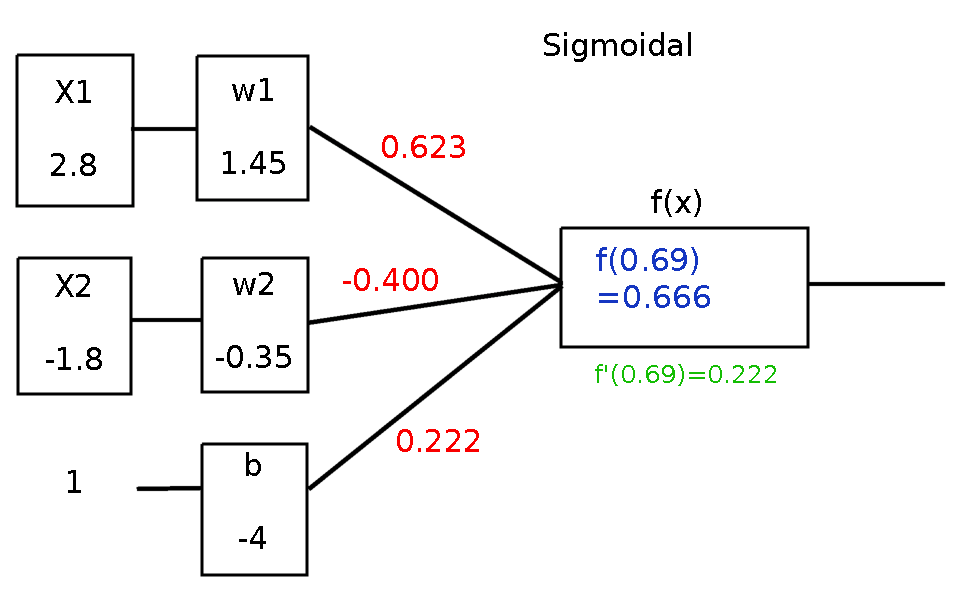
\includegraphics[width=0.5\textwidth]{Graphs/ejer1a.pdf}
                \end{center}
                \caption{1a}
                \label{fig:1a}
            \end{small}
        \end{figure}
        

    \item Hyperbolic tangent:
    \[  \tanh(x)
        \]

    Derivada:
    \[
        f'(x) =  \frac{1}{\cosh{x}^2} = 1 - \tanh^2x = 1 - f(x)^2
        \]

        \begin{figure}[H]
            \begin{small}
                \begin{center}
                    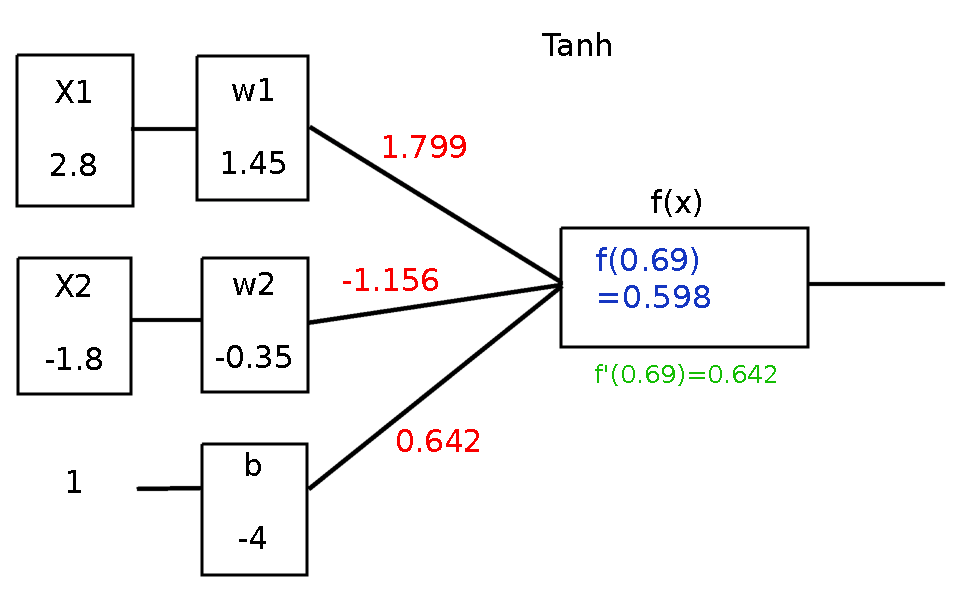
\includegraphics[width=0.5\textwidth]{Graphs/ejer1b.pdf}
                \end{center}
                \caption{1b}
                \label{fig:1b}
            \end{small}
        \end{figure}
        

    \item ELU:
    \[  f(x)=
        \begin{cases}
            x  & x \geq 0 \\
            \alpha(e^x - 1) & x < 0\\
        \end{cases}
        \]

    Derivada:

    \[ f'(x)=
        \begin{cases}
            1  & x \geq 0 \\
            \alpha e^x & x < 0\\
        \end{cases}
        \]

        \begin{figure}[H]
            \begin{small}
                \begin{center}
                    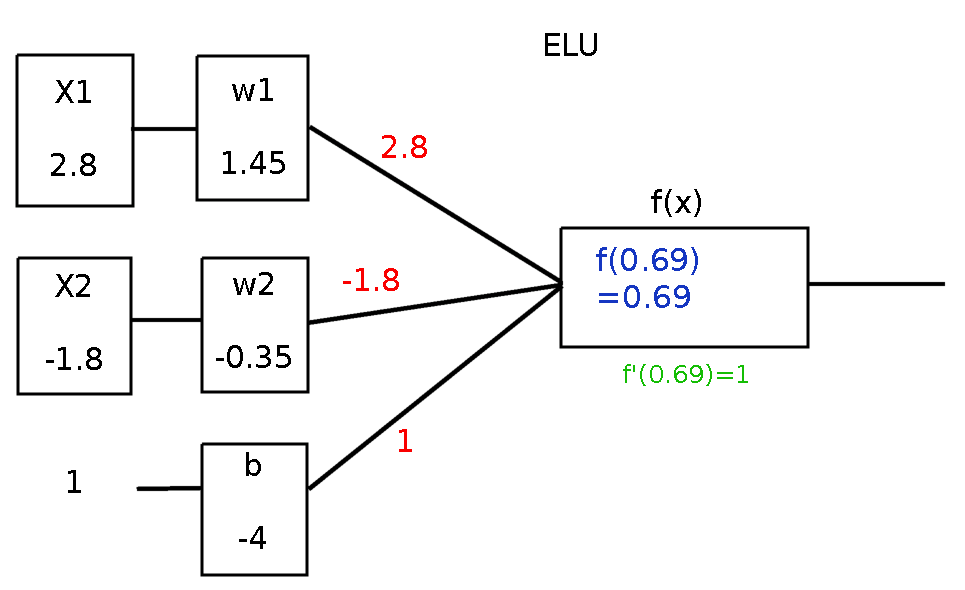
\includegraphics[width=0.5\textwidth]{Graphs/ejer1c.pdf}
                \end{center}
                \caption{1c}
                \label{fig:1c}
            \end{small}
        \end{figure}
        

    \item Leaky Relu:
    \[ f(x) = max(0.1x, x) =  \]
    \[ f'(x) =    \begin{cases}
                    0.1  & x < 0 \\
                    1    & x > 0\\
                 \end{cases}  \]

                 \begin{figure}[H]
                    \begin{small}
                        \begin{center}
                            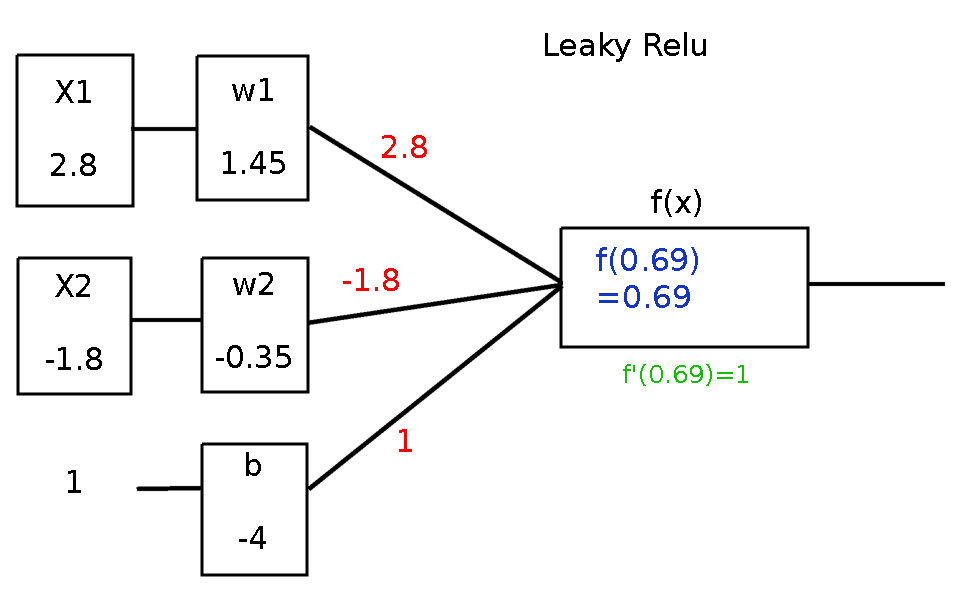
\includegraphics[width=0.5\textwidth]{Graphs/ejer1d.pdf}
                        \end{center}
                        \caption{1d}
                        \label{fig:1d}
                    \end{small}
                \end{figure}
                


\end{enumerate}

\section*{Ejercicio 2}

\begin{figure}[H]
    \begin{small}
        \begin{center}
            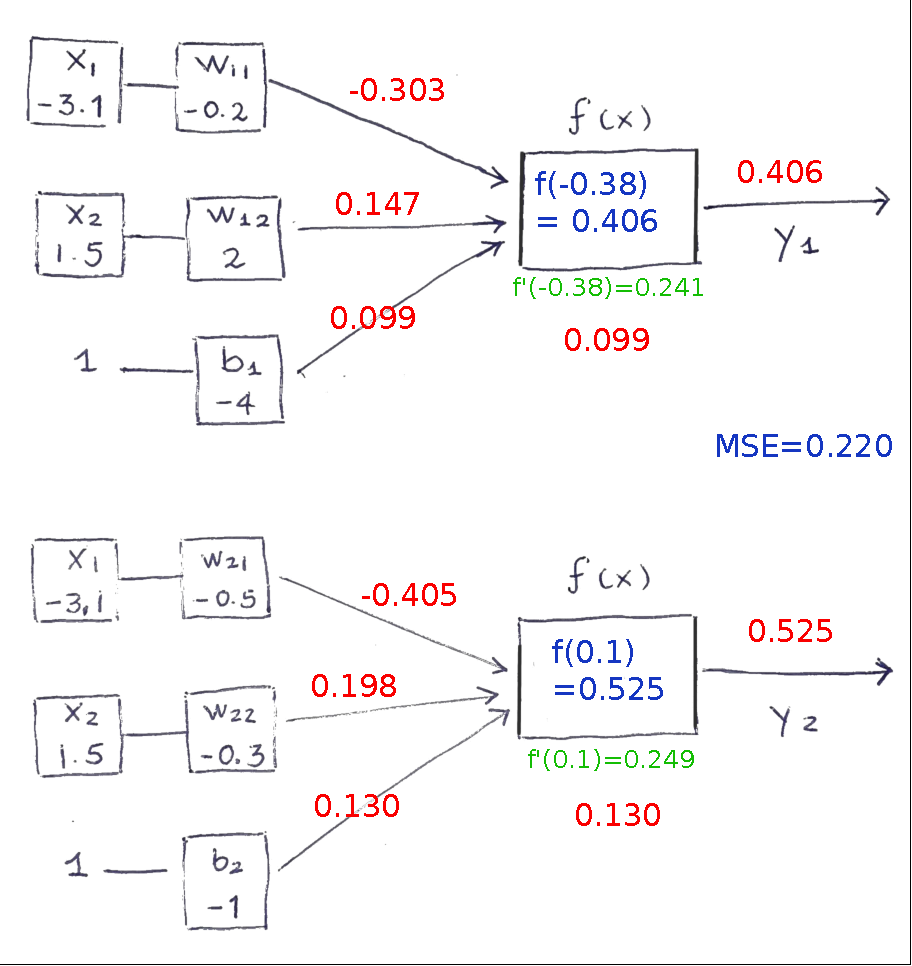
\includegraphics[width=0.5\textwidth]{Graphs/ejer2_grafico.pdf}
        \end{center}
        \caption{}
        \label{fig:}
    \end{small}
\end{figure}


\section*{Ejercicio 3}

\begin{figure}
    \begin{small}
        \begin{center}
            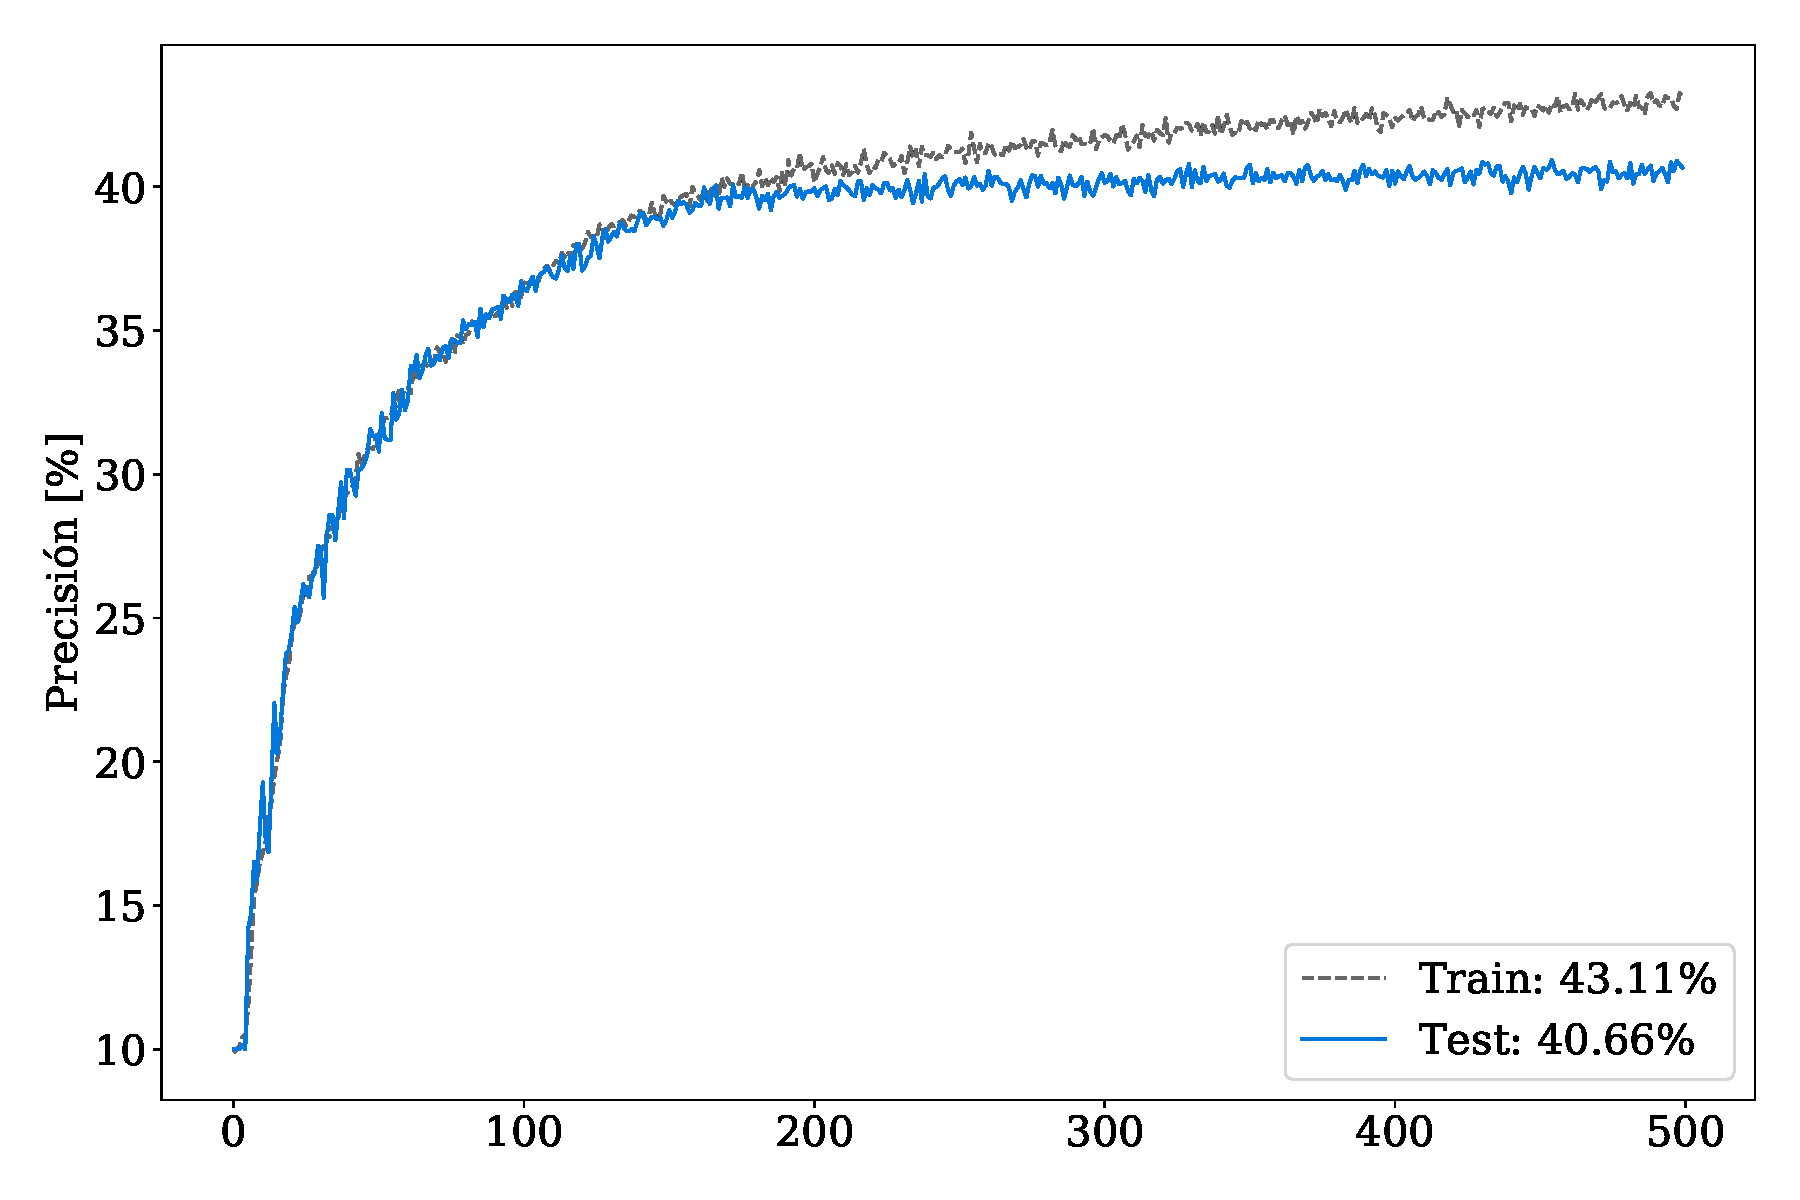
\includegraphics[width=0.5\textwidth]{Graphs/ejer3_acc.pdf}
        \end{center}
        \caption{}
        \label{fig:}
    \end{small}
\end{figure}


\begin{figure}
    \begin{small}
        \begin{center}
            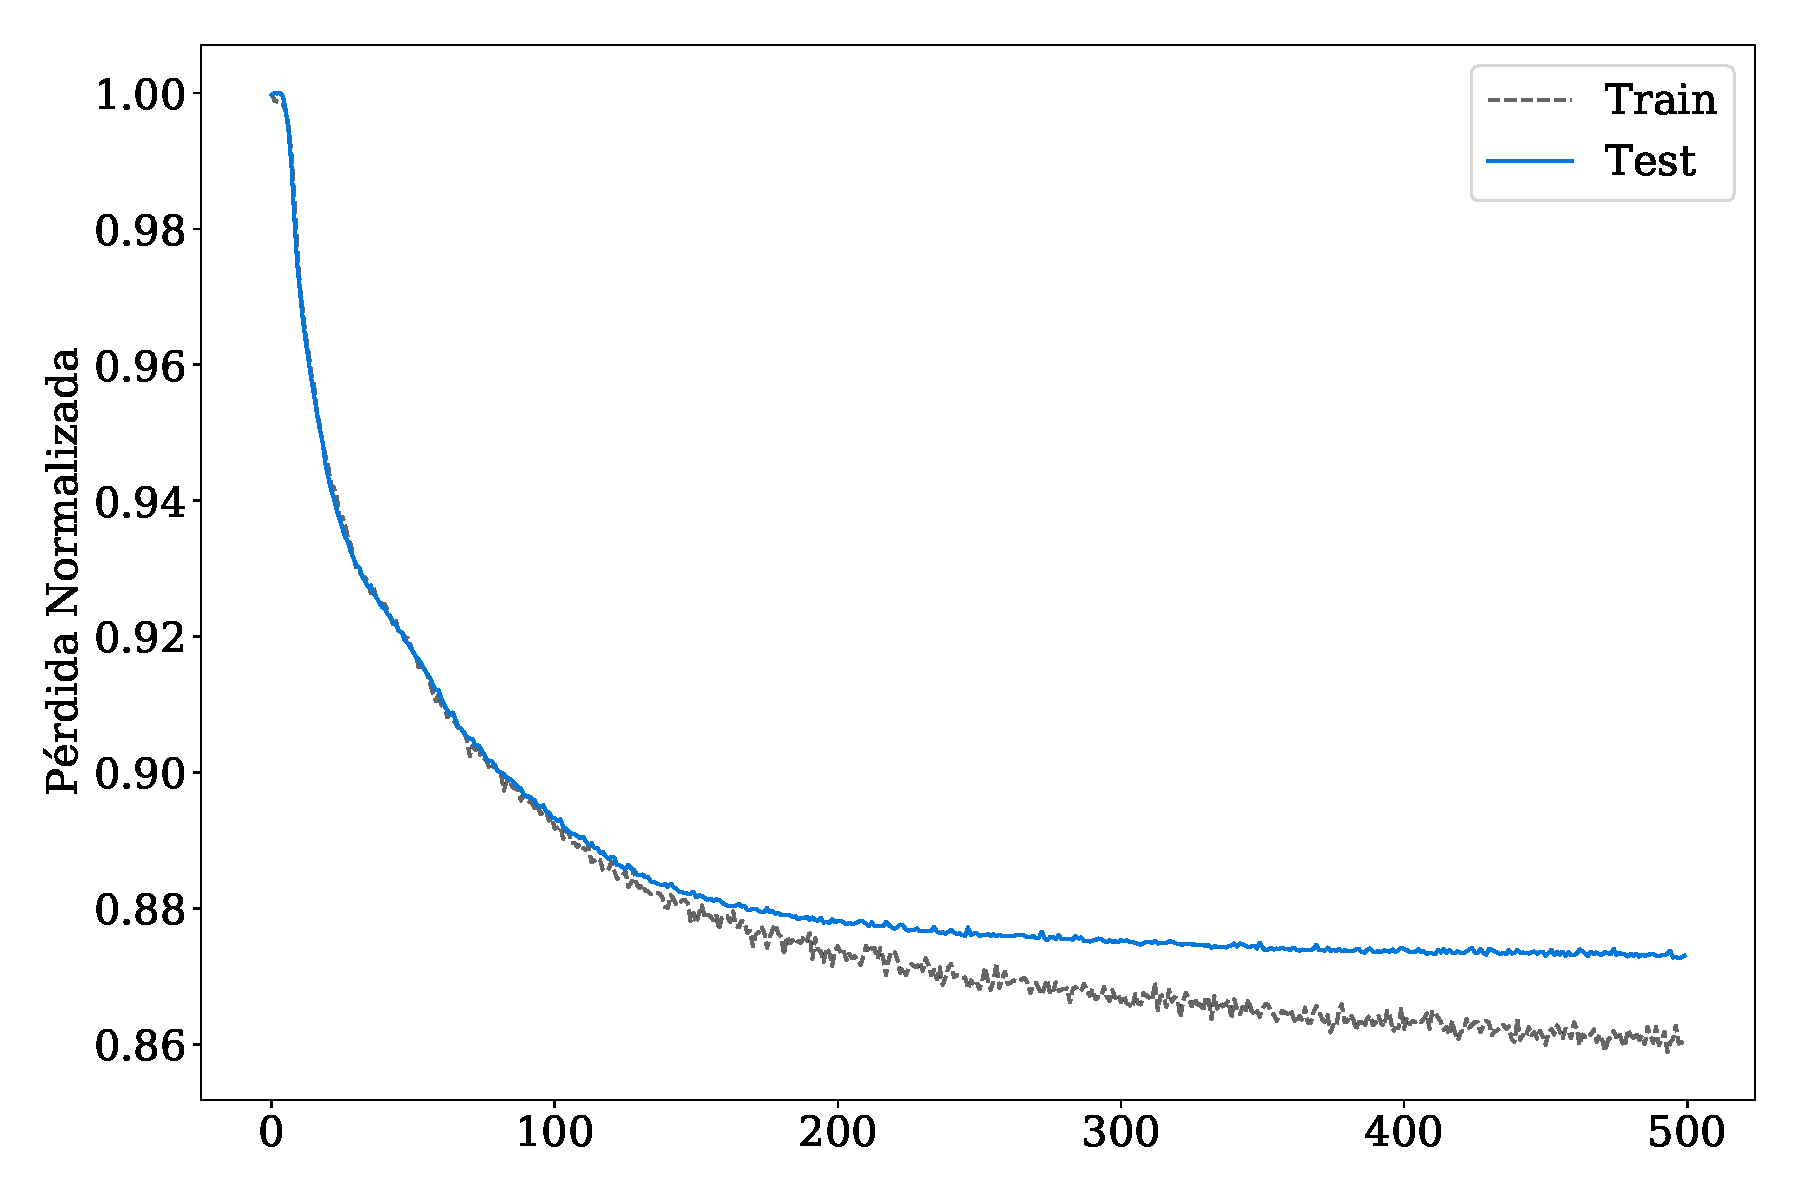
\includegraphics[width=0.5\textwidth]{Graphs/ejer3_loss.pdf}
        \end{center}
        \caption{}
        \label{fig:}
    \end{small}
\end{figure}



\section*{Ejercicio 4}

\section*{Ejercicio 5}

\section*{Ejercicio 6}

\begin{figure}[H]
    \centering
    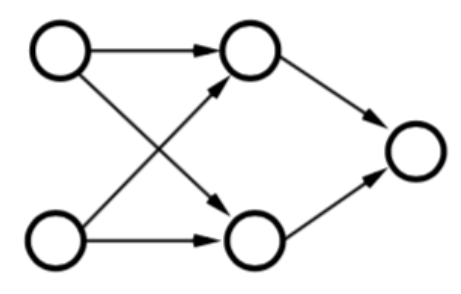
\includegraphics[width=0.4\textwidth]{Graphs/221.png}
    \caption{Arquitectura 221.}
    \label{fig:221}
\end{figure}


\begin{figure}[H]
    \centering
    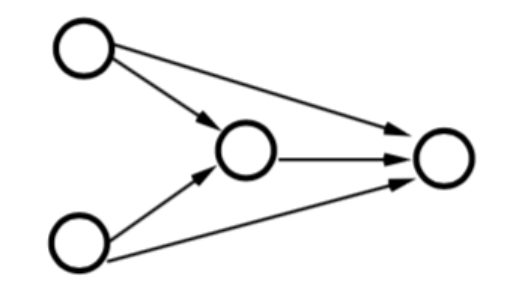
\includegraphics[width=0.4\textwidth]{Graphs/211.png}
    \caption{Arquitectura 211.}
    \label{fig:221}
\end{figure}


\section*{Ejercicio 7}

\begin{figure}[H]
    \centering
    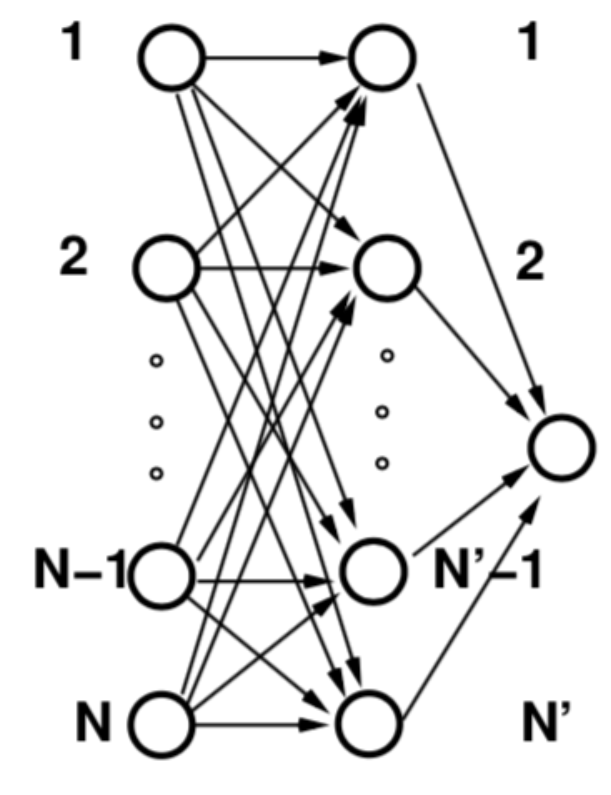
\includegraphics[width=0.4\textwidth]{Graphs/NN1.png}
    \caption{Arquitectura 211.}
    \label{fig:NN1}
\end{figure}

\section*{Ejercicio 8}

\end{document}